\chapter{Edit Filters as part of Wikipedia's socio-technical infrastructure}
\label{chap:filters}

%\section{Genesis}

``Abuse Filter is enabled'' reads the title of one of the eight stories of the March 23rd 2009 issue of English Wikipedia's newspaper, The Signpost~\cite{Signpost2009}.
``The extension allows all edits to be checked against automatic filters and heuristics, which can be set up to look for patterns of vandalism including page move vandalism and juvenile-type vandalism, as well as common newbie mistakes,'' the article proclaims.
%TODO something more from the signpost?

The extension, or at least its end user facing parts, was later renamed to ``edit filter'' in order to not characterise false positives as ``abuse'' and thus alienate good faith editors striving to improve the encyclopedia~\cite{Wikipedia:EditFilter},~\cite{Wikipedia:EditFilterTalkArchiveNameChange}.

In the present chapter, we aim to understand how edit filters work, who implements and runs them and above all, how and why they were introduced in the first place and what the qualitative difference is between them and other algorithmic quality control mechanisms.
%smth else we want to understand here?
%TODO come back at the end of the chapter and make sure, we answered these questions

\section{Data}

The foundations for the present chapter lie in EN Wikipedia's policies and guidelines.
Following pages were analysed in depth: \\
\url{https://en.wikipedia.org/wiki/Wikipedia:Edit_filter} \\
\url{https://en.wikipedia.org/wiki/Wikipedia_talk:Edit_filter/Archive_1} \\
<insert pages here>

%************************************************************************

\section{Definition}

According to EN Wikipedia's own definition, an edit filter is ``a tool that allows editors in the edit filter manager group to set controls mainly to address common patterns of harmful editing''~\cite{Wikipedia:EditFilter}.

A couple of keywords arouse interest here: %TODO make sure the chapter answered these questions
Who is in the edit filter manager group and how did they become part of it?
What controls exactly can be set?
What does ``mainly'' mean, are there other patterns addressed?
And what are the patterns of harmful editing addressed by the filters?

At least the ``mainly'' question is swiftly answered by the paragraph itself, since there is a footnote stating that ``[e]dit filters can and have been used to track or tag certain non-harmful edits, for example addition of WikiLove''~\cite{Wikipedia:EditFilter}.
We discuss (who is in) the edit filter manager group in section~\ref{section:who-can-edit} and the patterns of harmful editing (as well as some further non-harmful edit patterns) are inspected in detail in the next chapter.
Regarding the controls that can be set, we can briefly state that:
Every filter defines a regular expression pattern against which every edit made to Wikipedia is checked.
If there is a match, the edit in question is logged and potentially, additional actions such as tagging the edit summary, issuing a warning or disallowing the edit are invoked.
Both the regex patterns and the possible edit filter actions are investigated in greater detail in the following sections.

\subsection{Example of a filter}

For illustration purposes/better understanding, let us have a closer look at what a single edit filter looks like.
Edit filter with ID 365 is public and currently enabled (as of June 30th 2019).
This means the filter is working and everyone interested can view the filter's details.
Its description reads ``Unusual changes to featured or good content''.
The regex filter pattern is:
\begin{verbatim}
"page_namespace == 0 &
!(""confirmed"" in user_groups) &
old_size > 20000 & (
    ""#redirect"" in lcase(added_lines) |
    edit_delta < -15000 |
    edit_delta > 15000
) &
old_wikitext rlike
""\{\{([Ff]eatured|[Gg]ood)\s?article\}\}"""
\end{verbatim}
And the currently configured filter actions are: ``disallow''.

So, if a user whose status is not confirmed yet tries to edit a page in the article namespace which contains ``Featured'' or ``Good article'' and they either insert a redirect, delete 3/4 of the content or add 3/4 on top, the edit is automatically disallowed.

Note that an edit filter editor can easily change the action of the filter. (Or the pattern, as a matter of fact.)
The filter was last modified on October 23rd 2018.
All these details can be viewed on the filter's detailed page\footnote{\url{https://en.wikipedia.org/wiki/Special:AbuseFilter/365}}
or on the screenshot thereof (figure~\ref{fig:filter-details}) that I created for convenience.

Further information the filter detailed page displays is:
number of filter hits;
some statistics (the average time the filter takes to check an edit, percentage of hits and how many conditions from the condition limit it consumes);%TODO what is the condition limit
comments (left by filter editors, generally to log and explain changes);
flags (``Hide details of this filter from public view'', ``Enable this filter'', ``Mark as deleted'');
links to last modified (with diff and user who modified it), the edit filter's history and a tool for exporting the filter to another wiki;
and actions to take when the filter is triggered.

\begin{figure}
\centering
  \includegraphics[width=.9\paperwidth,height=.9\paperheight,keepaspectratio]{pics/detailed-page-filter365-no-boarder.png}
  \caption{Detailed page of edit filter \#365}~\label{fig:filter-details}
\end{figure}
%TODO graphic still looks weird..

%************************************************************************

\section{The AbuseFilter\footnote{Note that the user facing elements of this extention were renamed to ``edit filter'', however the extension itself, as well as its corresponding permissions, database tables etc. still reflect the original name.} Mediawiki extension}

At the end, from a technical perspective, Wikipedia's edit filters are a MediaWiki plugin that allows every edit (and some other editor's actions) to be checked against a speficied regular expression pattern before it is published.

Every time a filter is triggered, the action that triggered it as well as further data such as the user who triggered the filter, their IP address, and a diff of the edit (if it was an edit), a timestamp, the title of the page the user was looking at, etc. are logged.
Most frequently, edit filters are triggered upon new edits, there are however further editor's actions that can trip an edit filter.
As of June 30th 2019, these include: `edit', `move', `delete', `createaccount', `autocreateaccount', `upload', `stashupload'\footnote{See l. 181 in \url{https://gerrit.wikimedia.org/r/plugins/gitiles/mediawiki/extensions/AbuseFilter/+/refs/heads/master/includes/special/SpecialAbuseLog.php}}.
%TODO explain what the actions are, especially the less obvious ones such as `autocreateaccount'
Historically, further editor's actions such as `feedback', `gatheredit' and `moodbar' could trigger an edit filter.
However, this is no longer the case. %TODO explain why? I have the guess that these are not available in the software anymore (generally, not only for the edit filters)

When a filter is triggered, beside logging this, a further filter action may be invoked as well.
The plugin defines following possible filter actions:
`tag', `throttle', `warn', `blockautopromote', `block', `degroup', `rangeblock', `disallow'. (l.2808 in \url{https://gerrit.wikimedia.org/r/plugins/gitiles/mediawiki/extensions/AbuseFilter/+/refs/heads/master/includes/AbuseFilter.php})
%TODO verify that none of the actions are deprecated; I have my doubts that for instance `revoking auto-promoted groups' may not be available anymore
%TODO explain what each action means

The documentation page of the extension is here: \url{https://www.mediawiki.org/wiki/Extension:AbuseFilter}
and the code is hosted on gerrit, Wikimedia's git repository hosting service of choice: \url{https://gerrit.wikimedia.org/r/plugins/gitiles/mediawiki/extensions/AbuseFilter/+/refs/heads/master}.

The rules format can be viewed under \url{https://www.mediawiki.org/wiki/Extension:AbuseFilter/Rules_format}.

Data generated by the extension in stored in following database tables: \emph{abuse\_filter}, \emph{abuse\_filter\_log}, \emph{abuse\_filter\_action} and \emph{abuse\_filter\_history}~\cite{gerrit-abusefilter}.

Following new user permissions are introduced by the abuse filter plugin:
\begin{itemize}
    \item `abusefilter-modify': Modify abuse filters
    \item `abusefilter-view': View abuse filters
    \item `abusefilter-log': View the abuse log
    \item `abusefilter-log-detail':	View detailed abuse log entries
    \item `abusefilter-private': View private data in the abuse log
    \item `abusefilter-modify-restricted': Modify abuse filters with restricted actions
    \item `abusefilter-modify-global': Create or modify global abuse filters
    \item `abusefilter-revert':	Revert all changes by a given abuse filter
    \item `abusefilter-view-private': View abuse filters marked as private
    \item `abusefilter-log-private': View log entries of abuse filters marked as private
    \item `abusefilter-hide-log': Hide entries in the abuse log
    \item `abusefilter-hidden-log':	View hidden abuse log entries
    \item `abusefilter-private-log': View the AbuseFilter private details access log
\end{itemize}

%TODO: Flowchart of the filtering process!


%************************************************************************

\section{History}

Now that there is a general understanding of what edit filters look like today, let us take a step back and investigate how they came to be this way.
In order to understand the consensus building on the functionality of the extension, I sifted through the archives of the Edit Filter talk page\footnote{\url{https://en.wikipedia.org/w/index.php?title=Wikipedia_talk:Edit_filter/Archive_1&oldid=884572675}}
for the period between the announcement that the extension is planned up until the voting process preceding its introduction.
For a while at the beginnings of the discussion, there was some confusion among editors regarding the intended functionality of the EditFilter extension.
During the discussion(syn!), participating editors invoked various motivations for the introduction of the extension (which sometimes contradicted each other) and argued for or against the introduction depending on these.
The discussion (syn!) reflects a mix of ideological and practical concerns.
%TODO elaborate a bit on the different understandings of what the extension was supposed to do
The biggest controversies lay along the lines of filters being public-vs-private and the actions the filters were to invoke upon a match.
An automated rights revokation or block with no manual confirmation by a real person was of particular concern to a lot of editors.
As far as I am concerned, the later functionality was technically implemented but never really used (although there are `blockautopromote' actions triggered in the abuse\_filter\_log) %TODO investigate what exactly this means and why it hasn't happened since 2012

As to the public-vs-private debate, initially, it was planned that all filters are hidden from public view and only editors with special permissions (the edit filter managers) were supposed to be able to view and modify the patterns and logs.
The core developer of the extension was reasoning that its primary purpose was to fend off really persistent vandals with reasonable technical understanding who were ready to invest time and effort to circumvent anti-vandal measures
and that it was thus unwise to make circumvention easier to them by allowing them to view the pattern according to which their edits were supressed.
This was however met with serious resistence by the community who felt that such secret extension was contradicting Wikipedia's values of openness and transparency.
Besides, opponents of the filters being completely private were concerned that the tool was quite powerful and hiding stuff will prevent the community from monitoring (syn) for errors and abuse.

Although there were some diverging opinions on what the extension was supposed to target, in a nutshell, the motivation for its introduction seems to have been as follows:
bots weren't reverting some kinds of vandalism fast enough, or, respectively, these vandalism edits required a human intervention and took more than a single click to get reverted.
These were mostly obvious but pervasive cases of vandalism, possibly introduced in (semi-)automated fashion, that took some time and effort to clean up.
The motivation of the extention's developers was that if a filter just disallows such vandalism, vandal fighters could use their time for checking less obvious cases where more background knowledge/context is needed in order to decide whether an edit is vandalism or not.
The extention's developers felt that admins and vandal fighters could use this valuable time more productively.
According to the discussion archives, following types of edits were supposed to be targeted by the extension:\\
\url{https://en.wikipedia.org/wiki/Special:Contributions/Omm_nom_nom_nom}\\
%redirects to nonsensical names
\url{https://en.wikipedia.org/wiki/Special:Contributions/AV-THE-3RD}\\
\url{https://en.wikipedia.org/wiki/Special:Contributions/Fuzzmetlacker}\\

\begin{comment}
"It gives us the opportunity to lighten the hard restrictions we put on all users, instead placing tougher restrictions on those who are actually causing the problem.— Werdna talk 10:40, 25 June 2008 (UTC)"

// so there's general discontent with bots (bot governance) that has motivated the creation of this extention?
// the argument "bots are poorly tested and this is not is absurd before anything has happened."
// when was the BAG and the formal process there created?

"This extension has zero latency: when an edit pattern like this is detected, the account will be blocked instantly, with no time to cause disruption. Similarly, any questionable edit to the main page should incite a block-first-ask-questions-later approach. It's things like this that the extension is designed for, not to replace Clue Bot, VoABot, etc. I can make a personal promise that I will immediately remove any filter that triggers on the use of the word "nigger" - that would be foolish beyond belief. I could not agree more that secret settings are totaly incompatible with the wiki philosophy; but this extension is most definitely not. Happy‑melon 15:58, 2 July 2008 (UTC) "
// for the record, such filter exists and is active today, id=384

"This extension is designed to be used for vandals like the ones I link to below: intelligent, aggressive, destructive editors who aim to do as much damage as possible to the wiki and the people who edit it. It's not on the main field that we need this extension: the anti-vandal bots do a stunning job, and they do it at just the right level of efficiency. It's on the constant skirmishes against the handful of intelligent and malicious persistent vandals that we need every tool available just to stay ahead of their game. These are the editors who would, in the real world, be tried for crimes against humanity - the users who have demonstrated time and time again that all they want to do is do as much damage as possible. Do we allow ourselves to use prior restraint against them? No, because we don't need to - they've already done enough harm to condemn themselves many times over. Happy‑melon 21:07, 9 July 2008 (UTC)"

" And yet it's not good enough - within those few seconds, damage is caused that takes ten minutes or more to clear up. With this extension, we have zero latency: we can do the same job that's being done already, without having to have a user running a script on a paid-for server that has to fetch the block token every twenty seconds to make sure it can respond as fast as inhumanly possible; and we can do it instantly, cleanly, and without any fuss"

"I think here we need to remember what this extension is supposed to be used for: its primary advantage is that, being part of the site software, it has zero-latency: Misza13's anti-Grawp script can slam in a block token just 5 seconds after detecting a heuristic-matching edit pattern, but this extension can do it before the first vandal action has even been completed. It has no real advantages over anti-vandal bots other than speed and tidiness: the majority of its functions can be performed just as well by a well-written script running on an admin account. However, there are some functions, most notably rights changes, which are way beyond what an admin can imitate. I have a suspicion that a filter could easily be implemented to desysop any specific user on their next edit; or (worse still) desysop all admins as-and-when they edit. Even granting this permission only to bureucrats would be giving them a right that they don't currently have - full access to this extension gives users half the power of a steward. Consequently, the ability to set filters which invoke rights changes should, in my opinion, be assigned separately to the other permissions, and only to completely trusted users. I would say give it only to the stewards, but they do not have a local right on en.wiki that the extension can check; my second choice would be those already trusted to the level of 'oversight', which is essentially the ArbCom (and stewards if necessary). Everything else the extension offers can already be done by admins, and I can see no reason not to give them all the tools available. My personal preference, therefore, would be abusefilter-modify → 'sysop' and abusefilter-modify-rights → oversight. I'm especially keen to hear other people's views on this area. Happy‑melon 16:53, 29 June 2008 (UTC) "

Arguments for as restricted as possible, since 'there are precedents for disgruntled admins doing some leaking'; and motivated trolls can work an account up to admin; // I'm torn here though: every system can be abused; trolls can work accounts up to edit-filter-managers as well. So if that's our premise, we're lost from the beginning


%TODO: note on historically, all filters were supposed to be hidden
\end{comment}

%************************************************************************

\section{Building a filter: the internal perspective}
\subsection{How is a new filter introduced?}

The best practice way for introducing a new filter is described under \url{https://en.wikipedia.org/wiki/Wikipedia:Edit_filter/Instructions}.
According to the page, these steps should be followed:
\begin{itemize}
    \item read the docs: \url{https://www.mediawiki.org/wiki/Extension:AbuseFilter/Rules_format}
    \item test with debugging tools: \url{https://en.wikipedia.org/wiki/Special:AbuseFilter/tools} (visible only for users who are already in the edit filter managers user group)
    \item test with batch testing interface (dito)
    \item create logging only filter: \url{https://en.wikipedia.org/wiki/Special:AbuseFilter/new} (needs permissions)
    \item announce the filter at the edit filter notice board~\cite{Wikipedia:EditFilterNoticeboard}, so other edit filter managers can comment on it
    \item finally, fully enable the filter by adding an appropriate edit filter action.
\end{itemize}

Performance/efficiency seem to be fairly important for the edit filter system;
on multiple occasions, there are notes on recommended order of operations, so that the filter evaluates as resource sparing as possible~\cite{Wikipedia:EditFilterInstructions} or invitations to consider whether an edit filter is the most suitable mechanism for solving a particular issue at all~\cite{Wikipedia:EditFilter},~\cite{Wikipedia:EditFilterRequested}.


% Can filter editors introduce each filter they feel like introducing? Or is a community consensus due when a new filter is introduced?

Anyone can propose a new edit filter.
An editor who notices problematic/weird/.. behaviour they deem needs a filter can raise the issue at \url{https://en.wikipedia.org/wiki/Wikipedia:Edit_filter/Requested}.
The request can then be approved and implemented by an edit filter manager (mostly after a discussion/clarification of the details).
The Edit Filters Requests page also asks users to go through following checklist before requesting a filter:
\begin{itemize}
    \item "Filters are applied to all edits. Therefore, problematic changes that apply to a single page are likely not suitable for an edit filter."
    \item filters, after adding up, make editing slower
    \item in depth checks should be done by a separate software that users run on their own machines
    \item no trivial errors should be catched by filters (ala style guidelines)
    \item there are Titles Blacklist and Link/Spam Blacklist which should be used if the issue at hand has to do with a problematic title or link.
\end{itemize}


\subsection{Who can edit filters?}
\label{section:who-can-edit}

In order to be able to set up an edit filter on their own, an editor needs to have the \emph{abusefilter-modify} permission.
According to ~\cite{Wikipedia:EditFilter} this right is given only to editors who ``have the required good judgment and technical proficiency''.
Further down on the page it is clarified that it's administrators who can assign the permission to users (also to themselves) and they should only assign it to non-admins in exceptional cases, ``to highly trusted users, when there is a clear and demonstrated need for it''.
If editors wish to be given this permission, they can hone and prove their skills by helping with requested edit filters and false positives~\cite{Wikipedia:EditFilter}.

The formal process for requesting the \emph{abusefilter-modify} permission is to raise it to the edit filter noticeboard~\footnote{\url{https://en.wikipedia.org/wiki/Wikipedia:Edit_filter_noticeboard}}.
%TODO who can raise the issue to the noticeboard?
A discussion is held there, usually for 7 days, before a decision is reached~\cite{Wikipedia:EditFilter}.

A list of the current edit filter managers for the EN Wikipedia can be found here: \url{https://en.wikipedia.org/wiki/Special:ListUsers/abusefilter}.
As of May 10, 2019, there are 154 users in the ``edit filter managers'' group\footnote{\url{https://en.wikipedia.org/w/index.php?title=Special:ListUsers&offset=&limit=250&username=&group=abusefilter&wpsubmit=&wpFormIdentifier=mw-listusers-form}}.
(For comparison, as of March 9, 2019 there are 1181 admins, see \url{https://en.wikipedia.org/w/index.php?title=Special:ListUsers/sysop}.)
Out of the 154 edit filter managers only 11 are not administrators.

\begin{comment}
Quite some of the 154 edit filter managers have a kind of "not active at the moment" banner on their user page.
How many new editors have gotten the permission in recent time?
Otherwise the group is apparently aging..


CAT: https://ca.wikipedia.org/wiki/Especial:Usuaris/abusefilter (currently: 4 users)

-- auf Spanisch/Deutsch/Russisch existiert die Rolle nicht; interessant zu wissen, ob sie iwo subsumiert wurde
-- auf Bulgarisch übrigens auch nicht, aber da existiert auch die gesamte EditFilter seite nicht
Probably it's simply admins who can modify the filters there.
\end{comment}

\subsection{Modifying a filter}
% I may have found smth for theis subsection
It is not uncommon, that the action(s) a particular filter triggers change over time.
As of the guidelines for introducing new filters, every filter should be enabled in ``log only'' mode at the beginning.
After it has been deemed that the filter actually acts as desired, usually additional actions are switched on~\cite{Wikipedia:EditFilterInstructions}.
Sometimes, when a wave of particularly persistent vandalism arises, a filter is temporarily set to ``warn'' or ``disallow'' and the actions are removed again as soon as the filter is not tripped very frequently anymore. %TODO src? other than data?

\begin{comment}
this subsection used to describe a filter's detailed page; I moved all of it to "example of an edit filter". Not sure whether there is some significant information that by all means has to be included in this section in particular.
\end{comment}

\subsection{Urgent situations}

There are several provisions for urgent situations (which I think should be scrutinised extra carefully since ``urgent situations'' have historically always been an excuse for cuts in civil liberties).
For instance, generally, every new filter should be tested extensively in logging mode only (without any further actions) until a sufficient number of edits has demonstrated that it does indeed filter what it was intended to and there aren't too many false positives.
As a matter of fact, caution is solicited both on the edit filter description page~\cite{Wikipedia:EditFilter} and on the edit filter management page~\cite{Wikipedia:EditFilterManagement}.
Only then the filter should have ``warn'' or ``disallow'' actions enabled~\cite{Wikipedia:EditFilter}.
%TODO move this to the introducing a filter part, where it's mentioned for the first time that filters should be "log only" in the beginning; move verything else to further studies/long list of interesting questions
In ``urgent situations'' however (how are these defined? who determines they are urgent?), discussions about a filter may happen after it was already implemented and set to warn/disallow edits whithout thorough testing.
Here, the filter editor responsible should monitor the filter and the logs in order to make sure the filter does what it was supposed to~\cite{Wikipedia:EditFilter}.

%************************************************************************

\section{Filters during runtime: the external perspective}
\subsection{What happens when a filter gets triggered?}

There are several actions by editors that may trigger an edit filter.
Editing is the most common of them, but there are also filters targetting account creation, deletions, moving pages or uploading content\footnote{\url{https://www.mediawiki.org/wiki/Extension:AbuseFilter/Rules_format\#Variables_from_AbuseFilter}}.
%TODO src as a footnote or a proper ref?
% bzw think about how much of this is a unnecessary repetition and get rid of it

When an edit filter's regex pattern matches an editor's action, an entry is created in the \emph{abuse\_filter\_log} table and an additional action (or actions) may be invoked.
The documentation of the AbuseFilter extension provides us a complete list of the possible edit filter actions~\cite{Mediawiki:AbuseFilterActions}:
\begin{itemize}
    \item Logging: ``All filter matches are logged in the abuse log. This cannot be turned off.''
    \item Warning: ``The user is warned that their edit may not be appreciated, and is given the opportunity to submit it again. You may specify a specific system message containing the warning to display.'' A link to the false positives page~\cite{Wikipedia:EditFilterFalsePositives} is also provided. (the editor who tripped the filter is provided with the opportunity to revise their edit and re-submit it)
    \item Throttling: ``The filter will only match if a rate limit is tripped. You can specify the number of actions to allow, the period of time in which these actions must occur, and how those actions are grouped.
         The groupings are which sets of people should have aggregate (shared) throttles. That is, if you type "user", then the same user must match the filter a certain number of times in a certain period of time. You may also combine groups with commas to specify that throttle matches sharing all criteria will be aggregated. For example, using "ip,page", X filter matches in Y seconds from the same IP address to the same page will be required to trip the remainder of the actions.''
         (So this is something like, do this and that if a user edits a particular page X times for a Y period of time. In this sense: throttling always has to be paired with another action?)
    \item Disallowing: ``Actions matching the filter will be prevented, and a descriptive error message will be shown.'' The editor is provided the opportunity to report a false positive
    \item Revoking auto-promoted groups: ``Actions matching the filter will cause the user in question to be barred from receiving any extra groups from \$wgAutopromote for a period ranging from 3 to 7 days (random). This can be restored at the debug tools page.''
    \item Blocking: ``Users matching the filter will be blocked indefinitely, with a descriptive block summary indicating the rule that was triggered.''
    \item Removing from privileged groups: ``Users matching the filter will be removed from all privileged groups (sysop, bureaucrat, etc). A descriptive summary will be used, detailing the rule that was triggered.''
    \item Range-blocking: ``Somewhat of a "nuclear option", the entire /16 range from which the rule was triggered will be blocked for 1 week.''
    \item Tagging: ``The edit or change can be 'tagged' with a particular tag, which will be shown on Recent Changes, contributions, logs, new pages, history, and everywhere else. These tags are styleable, so you can have items with a certain tag appear in a different colour or similar.''
\end{itemize}

Range-blocking, blocking, removing from priviledged groups and revoking autopromoted groups haven't been used on the EN Wikipedia in recent years. %TODO: why? look for talk page archives around the last time they were used. Maybe there was a particular incident; nothing concerning autopromote in the EdiFilter talk page around 2012
To be more precise, the last time a filter action other than ``log only'', ``tag'', ``warn'' or ``disallow'' was triggered on the EN Wikipedia was in 2012. %TODO Refer to data analysis
There are two distinct filter actions in the \emph{abuse\_filter\_log} table: ``blockautopromote'' and ``aftv5flagabuse''.
% Following 4 filters have blockautopromote as an action (note that this could have changed since 2012!): 115, 267, 334, 21;
No idea what exactly they mean.

\begin{comment}
https://www.mediawiki.org/w/index.php?title=Extension:ArticleFeedbackv5&oldid=3136840

"The Article Feedback extension (aka Article Feedback Tool, Version 5) was a Wikimedia Foundation project designed to engage Wikimedia readers in the assessment of article quality, one of the five priorities defined in the strategic plan."

==============================================
https://www.mediawiki.org/w/index.php?title=Article_feedback/Version_5&oldid=2589150

"AFT5 was developed from November 2011 to June 2013, and tested in three pilots on the English, French and German Wikipedias. The goal of AFT5 was to engage readers to participate on Wikipedia -- and to help editors improve articles based on reader feedback. After careful review of pilot results, this project was discontinued in March 2014, as outlined below and in this report. "

"However, a majority of editors did not find reader comments useful enough to warrant the extra work of moderating this feedback"

//This would explain why all feedback filters were deleted
\end{comment}

Guidelines specifically call for careful use of ``disallow''.
Only severe cases for which ``substantially all good-faith editors would agree are undesirable'' or specific cases for which consensus has been reached should be disallowed~\cite{Wikipedia:EditFilter}.

\subsection{What happens when an editor triggers an edit filter? Do they notice this at all?}

As described in the previous section, a variety of different actions may occur when a filter gets tripped.
If a filter is set to ``warn'' or ``disallow'', the editor is notified that they hit a filter by a warning message (see~\ref{fig:screenshot-warn-disallow}).
These warnings describe the problem that occurred and present the editor with possible actions:
complain on the FalsePositives page (\url{https://en.wikipedia.org/wiki/Wikipedia:Edit_filter/False_positives}) in case of a disallow,
or, complain on the FalsePositives page and publish the change anyway in case of a warning.
(Of course, in case of a warning, the editor can modify their edit before publishing it.)
On the other hand, when the filter action is set to "tag" or "log" only, the editor doesn't really notice they tripped a filter unless they are looking more closely.
Tagged edits are marked as such in the page's revision history (see~\ref{fig:tags-in-history})
and all edits that trigger an edit filter are listed in the AbuseLog (\url{https://en.wikipedia.org/wiki/Special:AbuseLog}) (see~\ref{fig:screenshot-abuse-log}).
%TODO How about throttling

\begin{figure}
\centering
  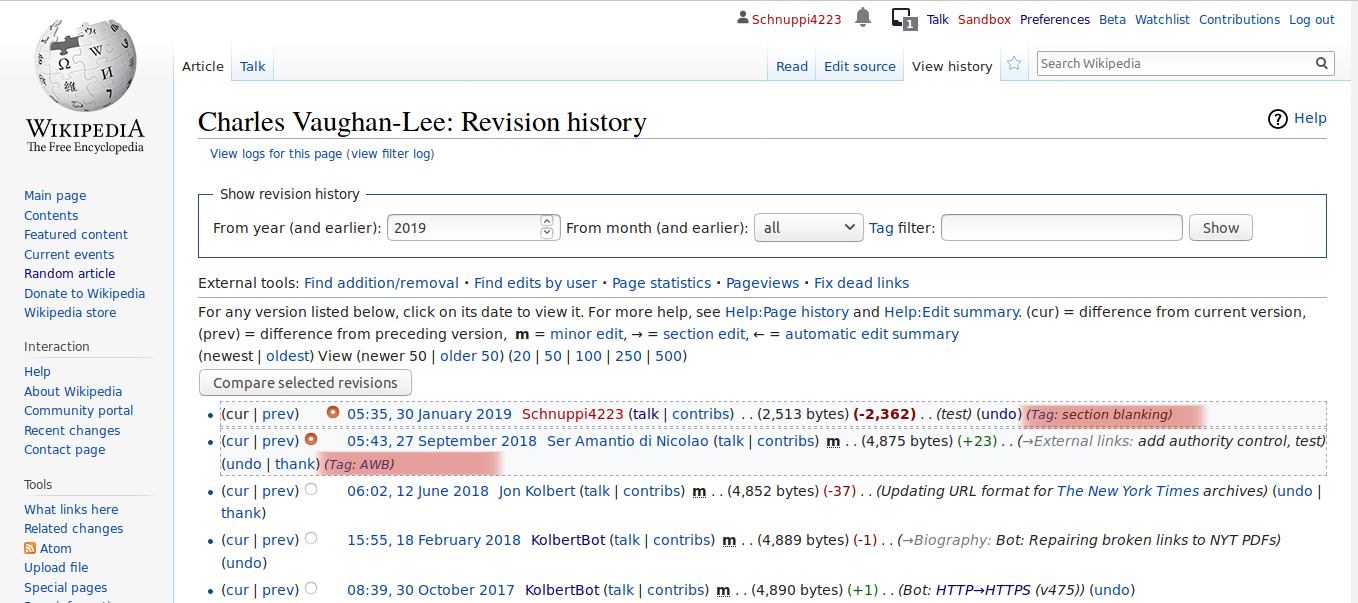
\includegraphics[width=0.9\columnwidth]{pics/screenshots-filter-trigger/Screenshot-tags-in-revision-history.png}
  \caption{Tagged edits are marked as such in a page's revision history}~\label{fig:tags-in-history}
\end{figure}

\begin{figure}
\centering
  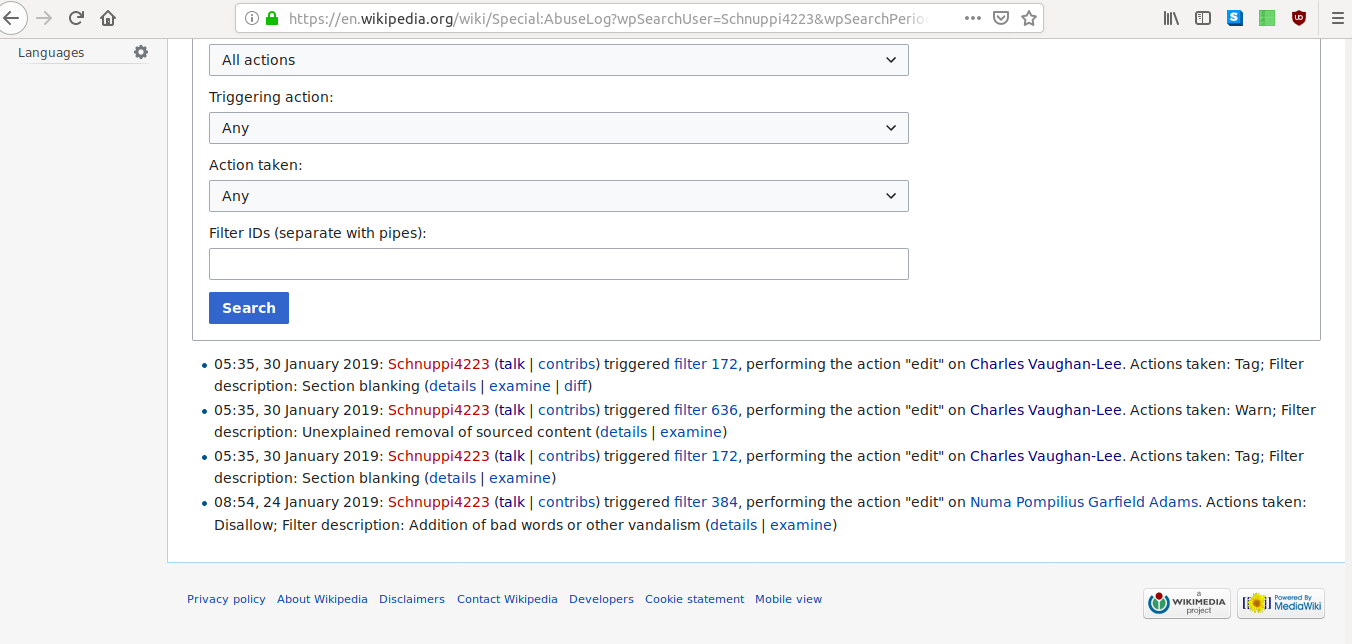
\includegraphics[width=0.9\columnwidth]{pics/screenshots-filter-trigger/Screenshot-abuse-log.png}
  \caption{Abuse Log showing all filter triggers by User Schnuppi4223}~\label{fig:screenshot-abuse-log}
\end{figure}

If the filter is set to disallow, a specific template is shown to the editor: "An automated filter has identified this edit as potentially unconstructive, so it has been disallowed. If this edit is constructive, please report this error. Disruptive editing may result in a block from editing."
"report this error" links to the FalsePositives page: \url{https://en.wikipedia.org/wiki/Wikipedia:Edit_filter/False_positives}
"block from editing" links to \url{https://en.wikipedia.org/wiki/Wikipedia:Blocking_policy}

The edit is not saved.

\begin{figure}
\centering
  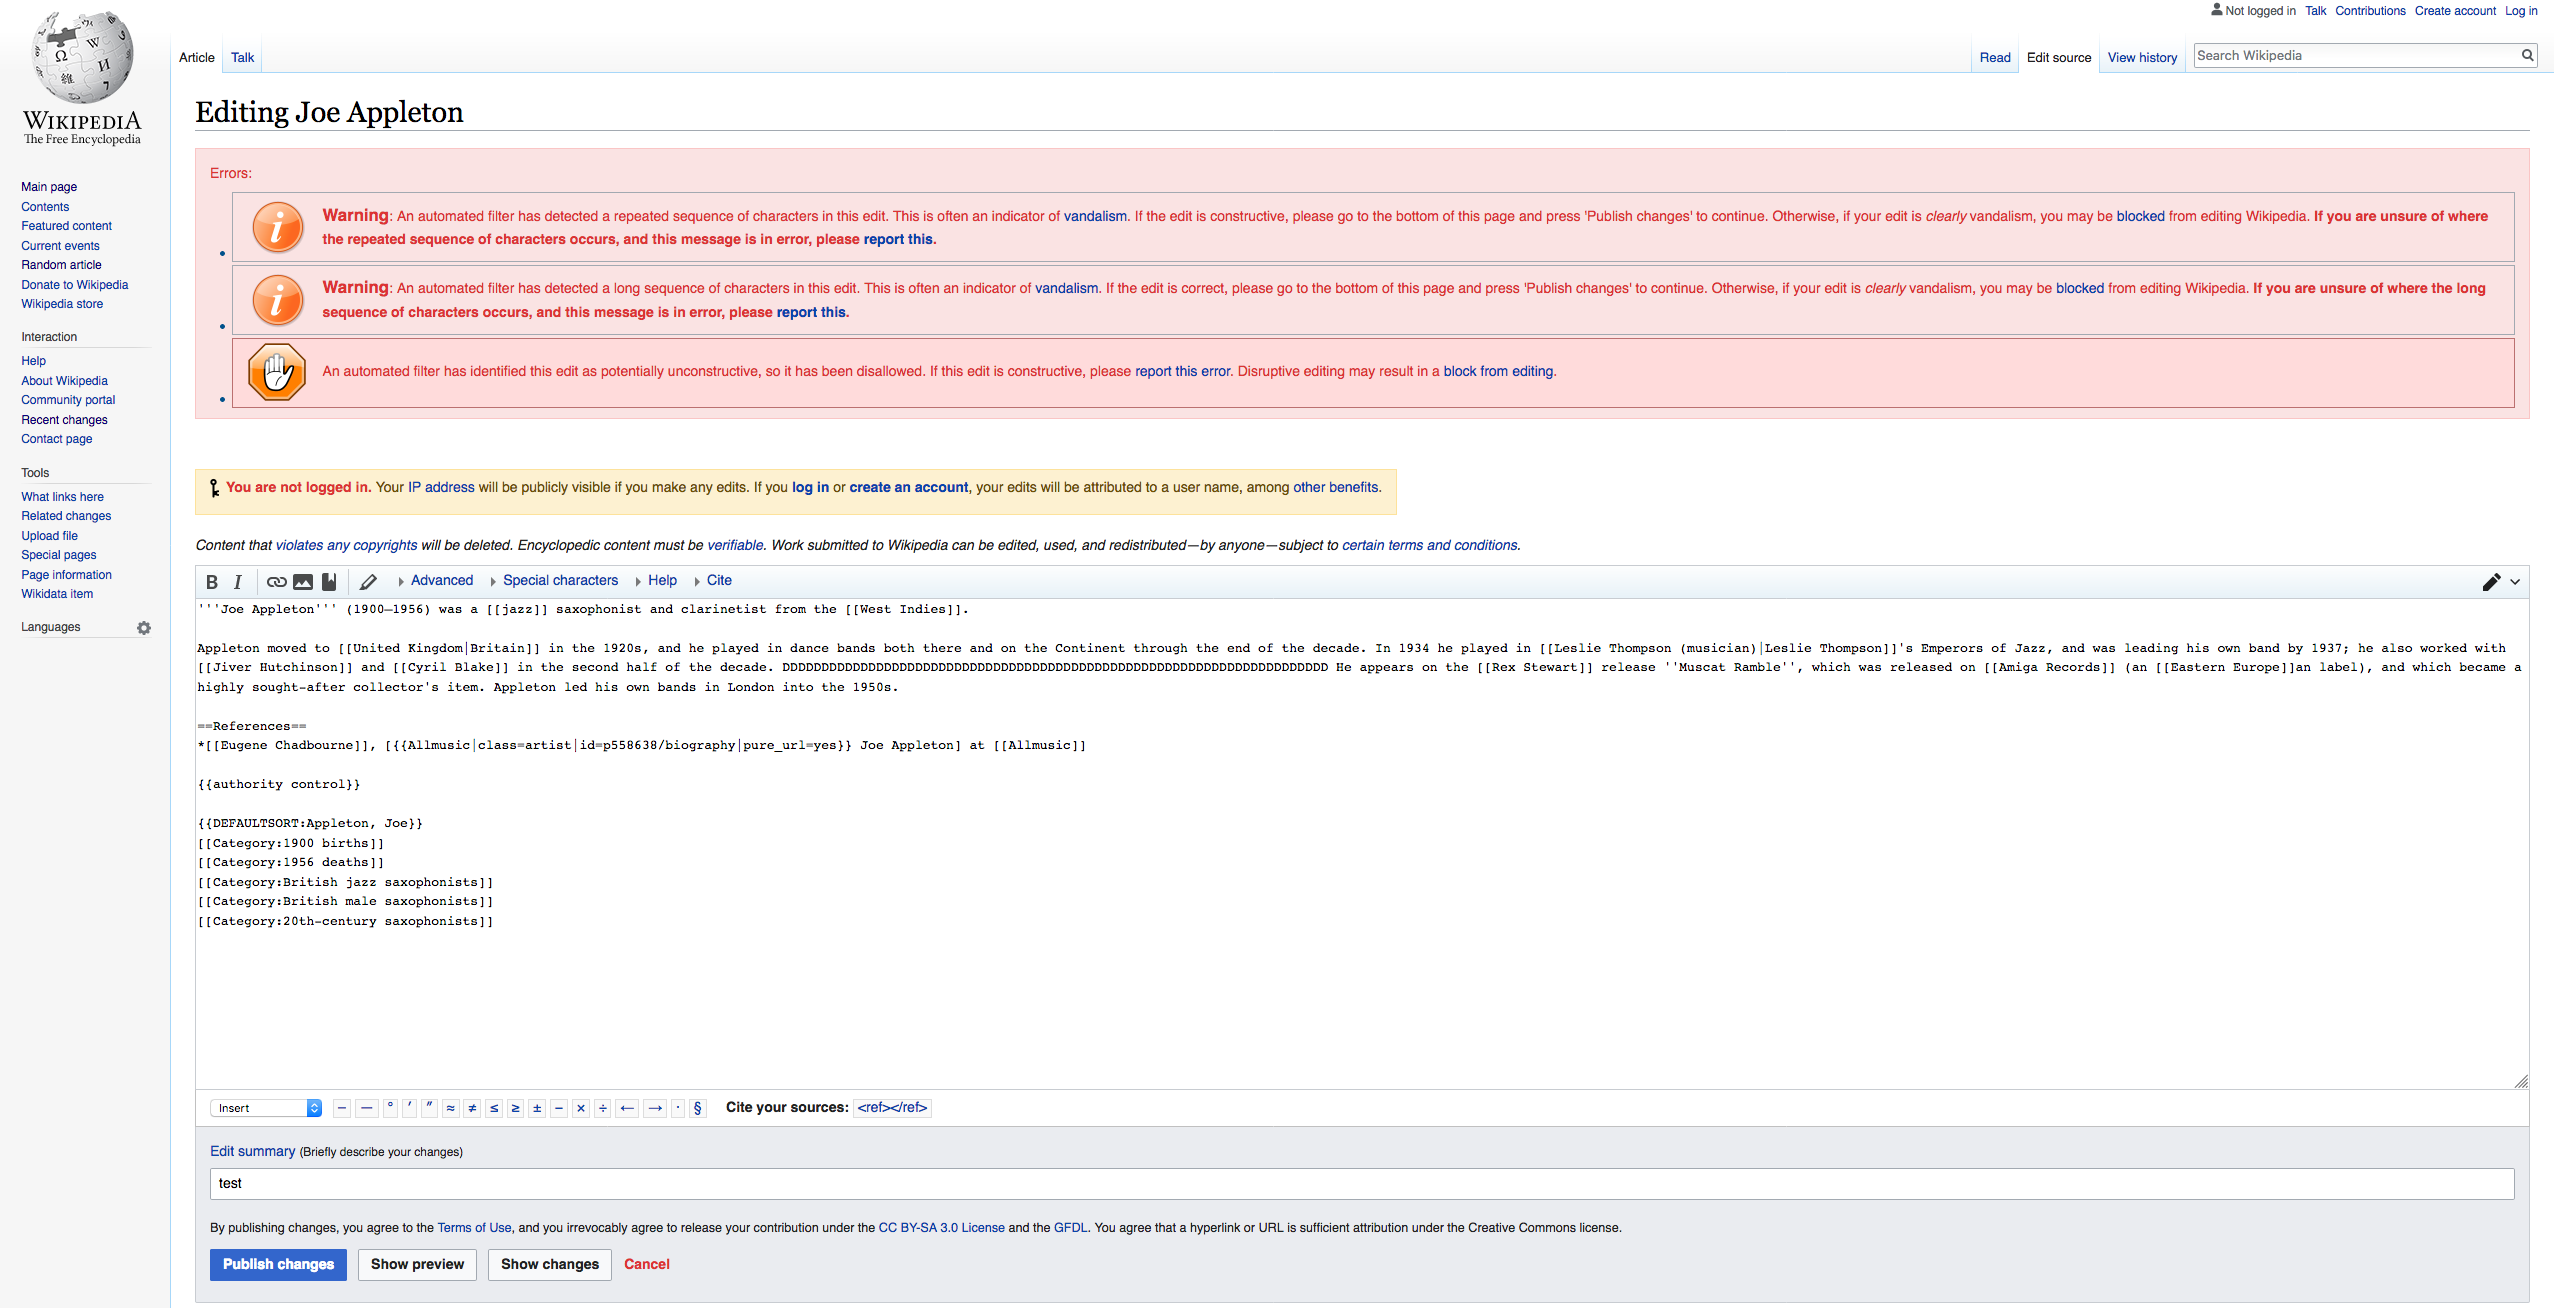
\includegraphics[width=0.9\columnwidth]{pics/screenshots-filter-trigger/Screenshot-trigger-warning-filter.png}
  \caption{Editor gets notified their edit triggered multiple edit filters}~\label{fig:screenshot-warn-disallow}
\end{figure}

\subsection{what happens afterwards}

If a user disagrees with the filter decision, they have the posibility of reporting a false positive
\url{https://en.wikipedia.org/wiki/Wikipedia:Edit_filter/False_positives}

\subsection{How are problems handled?}
%TODO review this part with presi: help to clear up the structure

There are several pages where problematic behaviour concerning edit filters as well as potential solutions are discussed.

For instance, current filters behaviour is discussed on the Edit Filter Noticeboard~\footnote{\url{https://en.wikipedia.org/wiki/Wikipedia:Edit_filter_noticeboard}}.
Issues handled here include changing the edit filter action of single filters, changing edit filter warning templates, problems with specific regexes or variables and proposals for filter deletions.
Furthermore, on the noticeboard discussions take place about giving edit filter manager rights to users, or withdrawing these if a misuse was observed and raising the issue with the editor directly didn't resolve the problem~\cite{Wikipedia:EditFilter}.

False positives among the filter hits are reported and discussed on a separate page~\footnote{\url{https://en.wikipedia.org/wiki/Wikipedia:Edit_filter/False_positives}}.
Edit filter managers monitor this page and improve filters based on true false positives, give advice to good faith editors who tripped a filter or discourage authors of vandalism edits to continue with them.
%TODO who moderates the false positives page? where does the info come from that it is edit filter managers?

Moreover, edit filter managers are advised to consult and comply with personal security best practices (such as choosing a strong password and using two-factor authentication).
If such an account is compromised, it loses its edit filter manager rights and gets blocked, since this threatens site security~\cite{Wikipedia:EditFilter}.

\begin{comment}
\url{https://en.wikipedia.org/wiki/Wikipedia:Edit_filter}
"In the unlikely event that your account is compromised, notify an administrator or bureaucrat (for administrators) immediately so they can block your account and remove any sensitive privileges to prevent damage. "
//interessanterweise is 2factor-auth auch nur für diese speziellen Benutzer*innen erlaubt; sonst kann man die Seite nicht ansehen
\end{comment}

%************************************************************************

\section{Edit filters' role in the quality control frame}

Let us review in this section what we have learnt so far and how edit filters fit in Wikipedia's quality control ecosystem.
%TODO: explain table with text

So, as shown in figure~\ref{fig:funnel-with-filters}, edit filters are crucial since they get active before any of the other mechanisms.

\begin{figure}
\centering
  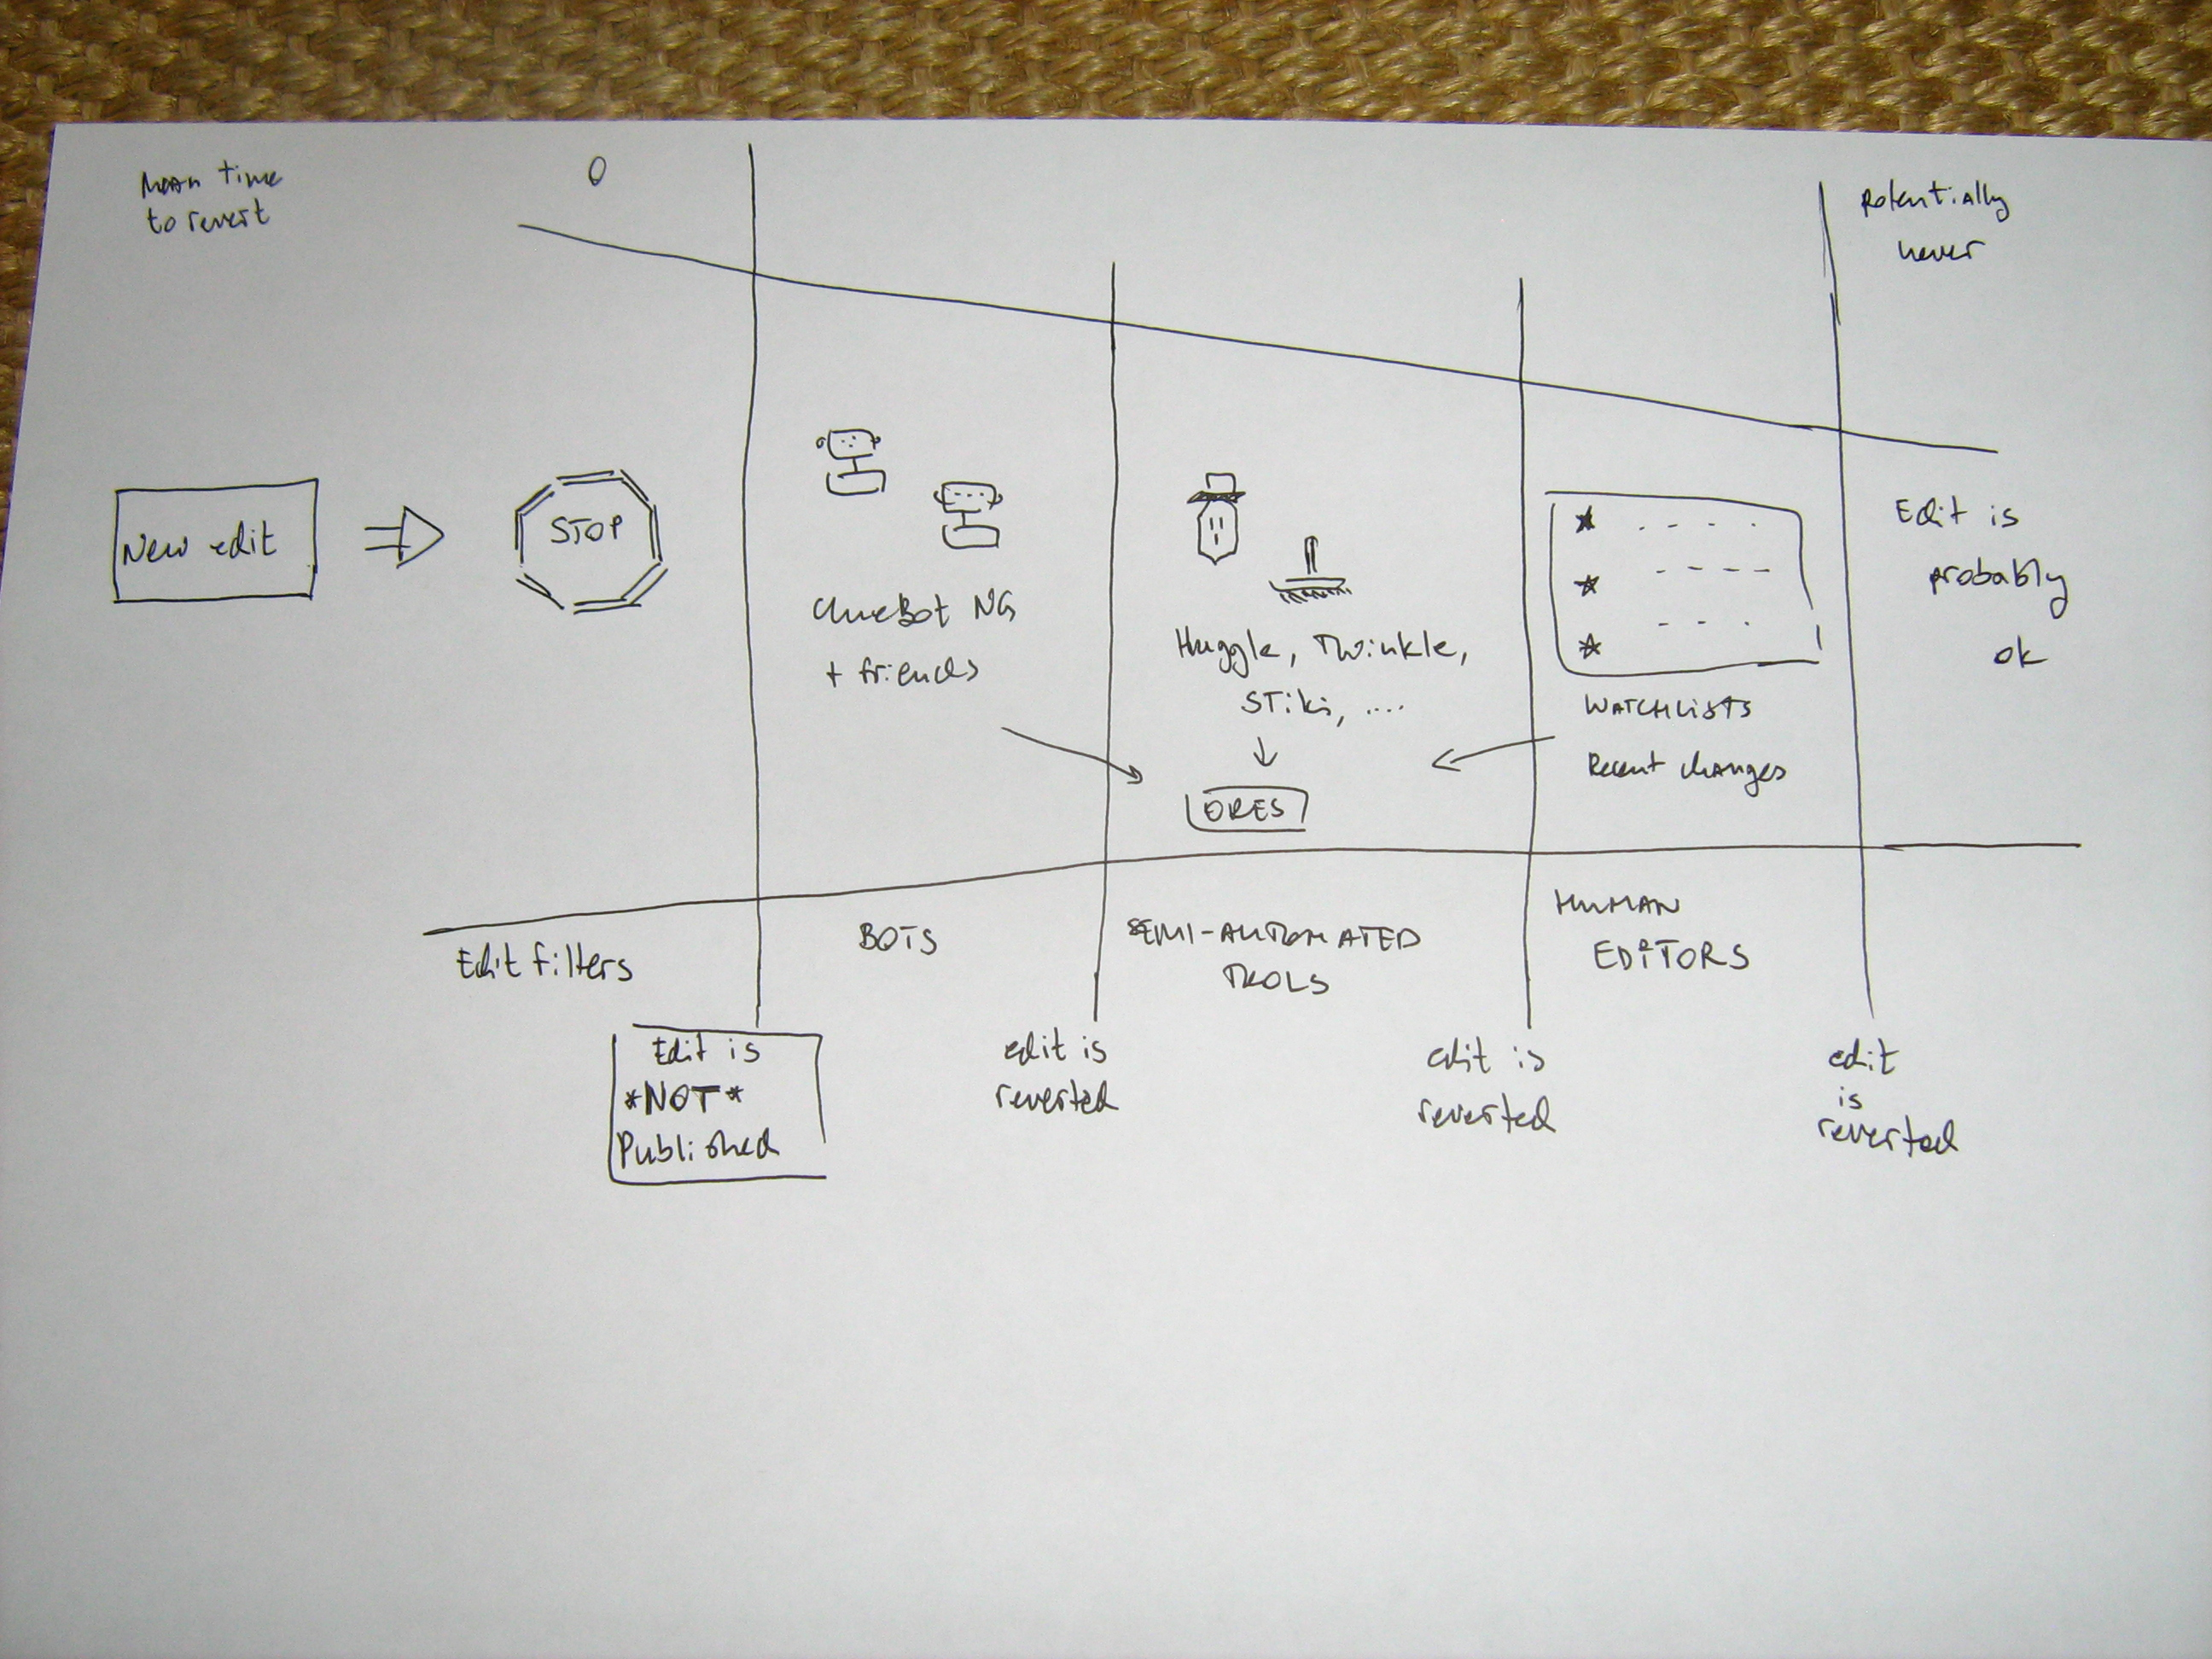
\includegraphics[width=0.9\columnwidth]{pics/funnel-diagramm-with-filters.JPG}
  \caption{Edit filters' role in the quality control frame}~\label{fig:funnel-with-filters}
\end{figure}

\begin{comment}
\begin{longtable}{ l | c | c | c | c }
    & Filters & Bots & Semi-Automated tools & ORES \\
\end{longtable}
\end{comment}

\begin{verbatim}
                     | Filters                          | Bots                          |  Semi-Automated tools   |  ORES
--------------------------------------------------------------------------------------------------------------------------------------------
                     |                                  |                               |                         |
                     | - based on REGEXes               | - rule/ML based               | - rule/ML based         | - ML framework
properties           | - part of the "software"/        | - "bespoke code": run on      | - heuristics obfusca-   | - not used directly, but can
                     |   platform (MediaWiki ext)       |   user's infrastructure       |   ted by the interface  |   instead be incorporated in
                     | - public filters are directly    | - no requirement for the code |   (but often configura- |   other tools
                     |   visible for everyone           |   to be made public           |   ble)                  |
                     |   interested                     | - you can relatively easily   | - mostly based on a     |
                     | - trigger *before* an edit is    |   get all the filters; you    |   centralised queue     |
                     |   published                      |   cannot easily get all bots  | - trigger after an edit |
                     | - source code of the extension   | - trigger after an edit is    |   is published          |
                     |   is publicly viewable           |   published                   |                         |
                     |                                  |                               |                         |
---------------------|------------------------------------------------------------------------------------------------------------------------
                     |                                  |                               |                         |
                     | - edit filter managers           | - no special persmissions/    | - *rollback* perm       | - mostly Scoring platform
                     |  group (EN Wiki)                 |   rights needed               |                         |   team (?)
Who does this?       |  (abusefilter-modify perm)       | - a bot gets a bot flag       |                         |
                     |                                  |                               |                         |
---------------------|------------------------------------------------------------------------------------------------------------------------
                     |                                  |                               |                         |
                     | - become an edit filter manager  | - get an approval to run the  | - learn the tool        | - understand ML
What are the hurdles | - you have to *only* understand  |   bot from the BAG            | - install Windows^^     | - formal requirements to
to participate       |   REGEXes (relatively simple?    | - programming knowledge       |   (some don't support   |   develop ORES?
                     |   although relatively fast quite | - understand APIs, ..         |   other OS)             |
                     |   confusing)                     | - (but there is a lot to      | - get the rollback perm |
                     |                                  |   understand with all the     |                         |
                     |                                  |   mechanisms)                 |                         |
                     |                                  |                               |                         |
-----------------------------------------------------------------------------------------------------------------------------------------------
                     |                                  |                               |                         |
                     | - censorship infrastructure?     | - "botophobia"                | - gamification          | - general ML concerns:
Concerns             | - powerful, can in theory block  |                               |                         |   hard to understand
                     |   editors based on hidden        |                               |                         |
                     |   filters                        |                               |                         |
                     |                                  |                               |                         |
------------------------------------------------------------------------------------------------------------------------------------------------
\end{verbatim}

\begin{comment}
From the Edit filter talk archives:
"Firstly, I must note that the code of the extension itself will be public in the MediaWiki subversion repository, that the filters will be editable by anyone with the appropriate privileges, and that it would be very simple to disable any user's use of the filtering system, any particular filter, or, indeed, the entire extension. This is quite different from, say, an anti-vandalism adminbot. The code is private, and, in any case, too ugly for anybody to know how to use it properly. The code can only be stopped in real terms if somebody blocks and desysops the bot, and the bot is controlled by a private individual, with no testing.

In this case, there are multiple hard-coded safeguards on the false positive rate of individual filters, and the extension itself will be well-tested. In addition, I suggest that a strong policy would be developed on what the filters can be used to do, and on what conditions they can match on: I've developed a little system which tests a filter on the last several thousand edits before allowing it to be applied globally."

    So, this claims that filters are open source and will be a collaborative effort, unlike bots, for which there is no formal requirement that the code is public (although in recent years, it kinda is, compare BAG and approval requirements).
    Also, the extension allows multiple users to work on the same filters and there are tests. Unlike bots, which are per definition operated by one user.

    "We're not targetting the 'idiots and bored kids' demographic, we're targetting the 'persistent vandal with a known modus operandi and a history of circumventing prevention methods' demographic. — Werdna • talk 07:28, 9 July 2008 (UTC)"

"It is designed to target repeated behaviour, which is unequivocally vandalism. For instance, making huge numbers of page moves right after your tenth edit. For instance, moving pages to titles with 'HAGGER?' in them. All of these things are currently blocked by sekrit adminbots. This extension promises to block these things in the software, allowing us zero latency in responding, and allowing us to apply special restrictions, such as revoking a users' autoconfirmed status for a period of time."
\end{comment}

\subsection{Alternatives to Edit Filters}

Since edit filters run against every edit saved on Wikipedia, it is generally adviced against rarely tripped filters and a number of alternatives is offered to edit filter managers and editors proposing new filters.
For example, there is the page protection mechanism that addresses problems on a single page.
Also, title and spam blacklists exist and these might be the way to handle problems with page titles or link spam~\cite{Wikipedia:EditFilter}.
Moreover, it is adviced to run in-depth checks (for single articles) separately, e.g. by using bots~\cite{Wikipedia:EditFilterRequested}.


\subsection{Collaboration with bots (and semi-automated tools)}

So far we have juxtaposed the single quality control mechanisms and compared them separetly.
It is however worth mentioning that they not only operate alongside each other but also cooperate on occasions.
%TODO see Geiger's paper (banning of a vandal?) where the process of tracing the same malicious editor throughout Wikipedia and reverting their eidts with various tools (and issuing them warnings) leads to the (temporary) block of the editor

For instance, DatBot~\cite{Wikipedia:DatBot} monitors the abuse log\footnote{\url{https://en.wikipedia.org/wiki/Special:AbuseLog}}
and reports users tripping certain filters to WP:AIV (Administrator intervention against vandalism)\footnote{\url{https://en.wikipedia.org/wiki/Wikipedia:Administrator_intervention_against_vandalism}} and WP:UAA (usernames for administrator attention)\footnote{\url{https://en.wikipedia.org/wiki/Wikipedia:Usernames_for_administrator_attention}}.
It is the successor of Mr.Z-bot\footnote{\url{https://en.wikipedia.org/wiki/User:Mr.Z-bot}}.
which used to report users from the abuse log to WP:AIV, but has been inactive since 2016 and therefore recently deactivated.
%\url{https://en.wikipedia.org/wiki/Wikipedia:Bots/Requests_for_approval/Mr.Z-bot_7}
%TODO are there further examples of such collaborations: consider scripting smth that parses the bots descriptions from https://en.wikipedia.org/wiki/Category:All_Wikipedia_bots and looks for "abuse" and "filter"

\begin{comment}
    https://en.wikipedia.org/wiki/User:MusikBot/FilterMonitor
    "Reports functional changes of edit filters to the watchable page User:MusikBot/FilterMonitor/Recent changes. The template {{recent filter changes}} formats this information and can be transcluded where desired."

    https://en.wikipedia.org/wiki/User:MusikBot/StaleFilters
    "StaleFilters: Reports enabled filters that have not had any hits in over 30 days, as specified by /Offset. "

    https://en.wikipedia.org/wiki/User:MusikBot/AbuseFilterIRC
    "AbuseFilterIRC: Relays all edit filter hits to IRC channels and allows you to subscribe to notifications when specific filters are tripped. See #wikipedia-en-abuse-log-all connect for the English Wikipedia feed. "
\end{comment}

Apparently, Twinkle at least has the possibility of using heuristics from the abuse filter log for its queues.
% is that so? the only place I can find abuse filters mentioned with Twinkle is in the source code: https://github.com/azatoth/twinkle/blob/master/morebits.js#L2636; and I'm not quite sure what this part of the code does.
\begin{comment}
%TODO check other tools

So, Huggle let the user define their own queue, but only along predefined parameters. So it's not really possible right now to hook it up to the AbuseLog
\end{comment}

\begin{comment}
    Not sure where this fits in
\subsection{TOR}
(Interesting side note: editing via TOR is disallowed altogether: "Your IP has been recognised as a TOR exit node. We disallow this to prevent abuse" or similar, check again for wording. Compare: "Users of the Tor anonymity network will show the IP address of a Tor "exit node". Lists of known Tor exit nodes are available from the Tor Project's Tor Bulk Exit List exporting tool." \url{https://en.wikipedia.org/wiki/Wikipedia:Vandalism})

Here is where this comes from:
https://www.mediawiki.org/wiki/Extension:TorBlock
"The TorBlock extension automatically applies restrictions to Tor exit node's access to the wiki's front-door server."

TorNodeBot https://en.wikipedia.org/wiki/User:TorNodeBot
    Tasks:
    TorNodeBot is a bot that monitors the Tor network and ensures that Wikipedia exit nodes (those nodes in the Tor network that can be the last "hop" and route data to its final destination) can not edit, in accordance with our policy on Open proxies. The TorBlock extension is supposed to handle this automatically, but tends to miss several exit nodes and goes down on occasion. TorNodeBot fills in the gaps left open by the extension. This bot runs continuously and applies blocks when all of the following 3 conditions are met:

        The node is present in the Tor directory service as an exit node router
        The node is responding to requests and can route to Wikipedia's sandbox
        The node is not blocked already by the TorBlock extension

When all three of these conditions are met, a temporary block is placed on the node.

\end{comment}

Timeline
\begin{longtable}{ r | p{.8\textwidth}}
   Oct 2001 & automatically import entries from Easton’s Bible Dictionary by a script \\
29 Mar 2002 & First version of \url{https://en.wikipedia.org/wiki/Wikipedia:Vandalism} (WP Vandalism is published) \\
   Oct 2002 & RamBot \\
       2006 & BAG was first formed \\
13 Mar 2006 & 1st version of Bots/Requests for approval is published: some basic requirements (also valid today) are recorded \\
28 Jul 2006 & VoABot II ("In the case were banned users continue to use sockpuppet accounts/IPs to add edits clearly rejected by consensus to the point were long term protection is required, VoABot may be programmed to watch those pages and revert those edits instead. Such edits are considered blacklisted. IP ranges can also be blacklisted. This is reserved only for special cases.") \\
21 Jan 2007 & Twinkle Page is first published (empty), filled with a basic description by beginings of Feb 2007 \\
24 Jul 2007 & Request for Approval of original ClueBot \\
16 Jan 2008 & Huggle Page is first published (empty) \\
18 Jan 2008 & Huggle Page is first filled with content \\
23 Jun 2008 & 1st version of Edit Filter page is published: User:Werdna announces they're currently developing the extention \\
 2 Oct 2008 & \url{https://en.wikipedia.org/wiki/Wikipedia_talk:Edit_filter} was first archived; its last topic was the voting for/against the extention which seemed to have ended end of Sep 2008 \\
   Jun 2010 & STiki initial release \\
20 Oct 2010 & ClueBot NG page is created \\
11 Jan 2015 & 1st commit to github ORES repository \\
30 Nov 2015 & ORES paper is published
\end{longtable}

* look at Timeline: the time span in which vandal fighting bots/semi-automated tools and then edit filters were introduced, fits logically into the process after the exponential growth of Wikipedia took off and it was no more the small group that could handle things but suddenly had to face a huge workload which wasn't feasible without technical support.
* in consecuence, edits of a lot of newcomers from that time were reverted stricter than before (with the help of the automated tools) which drove a lot of them away

%************************************************************************

\section{Fazit}
%Conclusion, resume, bottom line

In short, in this chapter we found/worked out following salient characteristics of edit filters: ....
Why does this system continue to exist in times of fancier (syn!) machine learning based tools?


maybe it's a historical phenomenon (in many regards):
* perhaps there were differences that are not essential anymore, such as:
  * on which infrastructure does it run (part of the core software vs own computers of the bot operators)
  * filters are triggered *before* an edit is even published, whereas bots (and tools) can revert an edit post factum. Is this really an important difference in times when bots need a couple of seconds to revert an edit?
* perhaps the extension was implemented because someone was capable of implementing and working well with this type of systems so they just went and did it (do-ocracy; Wikipedia as a collaborative volunteer project);
* perhaps it still exists in times of fancier machine learning based tools (or bots) because rule-based systems are more transparent/easily understandable for humans and writing a regex is simpler than coding a bot.
* hypothesis: it is easier to set up a filter than program a bot. Setting up a filter requires "only" understanding of regular expressions. Programming a bot requires knowledge of a programming language and understanding of the API.

Question:
Oftentimes edit filter managers are also bot operators; how would they decide when to implement a filter and when a bot?
%TODO: ask people! (on IRC?)
I've compiled a list of edit filter managers who are simultaneously also bot operators;
I've further assembled the bots they run and made notes on the bots that seem to be relevant to vandalism prevention/quality assurance
I'm currently trying to determine from document traces what filter contributions the corresponding edit filter managers had and whether they are working on filters similar to the bots they operate.
Insight is currently minimal, since abuse\_filter\_history table is not available and we can only determine what filters an edit filter manager has worked on from limited traces such as: last modifier of the filter from abuse\_filter table; editors who signed their comments from abuse\_filter table; probably some noticeboards or talk page archives, but I haven't looked into these so far.

%TODO make sure the questions at l.12 and l.28 are answered

\begin{comment}
\url{http://www.aaronsw.com/weblog/whorunswikipedia}
"But what’s less well-known is that it’s also the site that anyone can run. The vandals aren’t stopped because someone is in charge of stopping them; it was simply something people started doing. And it’s not just vandalism: a “welcoming committee” says hi to every new user, a “cleanup taskforce” goes around doing factchecking. The site’s rules are made by rough consensus. Even the servers are largely run this way — a group of volunteer sysadmins hang out on IRC, keeping an eye on things. Until quite recently, the Foundation that supposedly runs Wikipedia had no actual employees.
This is so unusual, we don’t even have a word for it. It’s tempting to say “democracy”, but that’s woefully inadequate. Wikipedia doesn’t hold a vote and elect someone to be in charge of vandal-fighting. Indeed, “Wikipedia” doesn’t do anything at all. Someone simply sees that there are vandals to be fought and steps up to do the job."
//yeah, I'd call it "do-ocracy"

Reflections on the archive discussion
So, to summarise once again. Problem is blatant vandalism, which apparently doesn't get reverted fast enough.
Human editors are not very fast in general and how fast it is solving this with a bot depends on how often the bot runs and what's its underlying technical infrastructure (e.g. I run it on my machine in the basement which is probably less robust than a software extension that runs on the official Wikipedia servers).

\end{comment}

\begin{comment}
Can I answer these questions?

* Why are there mechanisms triggered before an edit gets published (such as edit filters), and such triggered afterwards (such as bots)? Is there a qualitative difference?
* I want to help people to do their work better using a technical system (e.g. the edit filters). How can I do this?
* The edit filter system can be embedded in the vandalism prevention frame. Are there other contexts/frames for which it is relevant?

* stick to research questions from Confluence, they are already carefully crafted and narrowed down as appropriate
  Q1 We wanted to improve our understanding of the role of filters in existing algorithmic quality-control mechanisms (bots, ORES, humans).
  Q2 Which type of tasks do these filters take over in comparison to the other mechanisms? How these tasks evolve over time (are they changes in the type, number, etc.)?
  Q3 Since filters are classical rule-based systems, what are suitable areas of application for such rule-based system in contrast to the other ML-based approaches.
\end{comment}
